%==============================================================================
%  Laporan Tugas Besar IF2224 - Teori Bahasa Formal dan Automata
%  Milestone 4 : Intermediate Code and Interpreter
%  Kelompok CNA - Arion Compiler
%
%  Berkas utama. Struktur laporan dibuat modular: tiap bab berada pada berkas
%  terpisah di dalam folder "bagian/" dan disisipkan dengan \input.
%==============================================================================
\documentclass[11pt,a4paper]{article}

%------------------------------------------------------------------ Encoding
\usepackage[utf8]{inputenc}
\usepackage[T1]{fontenc}
\usepackage[bahasa]{babel}

%------------------------------------------------------------------ Tata letak
\usepackage[margin=2.5cm]{geometry}
\usepackage{setspace}
\onehalfspacing
\usepackage{parskip}

%------------------------------------------------------------------ Visual & tabel
\usepackage{graphicx}
\usepackage[table]{xcolor}
\usepackage{colortbl}
\usepackage{booktabs}
\usepackage{tabularx}
\usepackage{longtable}
\usepackage{array}
\usepackage{float}
\usepackage{caption}
\usepackage{enumitem}
\usepackage{amsmath}
\usepackage{amssymb}
\usepackage[most]{tcolorbox}
\usepackage{titlesec}
\usepackage{tikz}
\usetikzlibrary{shapes.geometric, arrows.meta, positioning, calc}
\usepackage{listings}

%------------------------------------------------------------------ Hyperref (terakhir)
\usepackage[colorlinks=true, linkcolor=biruITB, urlcolor=biruITB, citecolor=biruITB]{hyperref}

%------------------------------------------------------------------ Palet warna
\definecolor{biruITB}{RGB}{0,80,158}
\definecolor{hijauJudul}{RGB}{46,125,50}
\definecolor{abuKode}{RGB}{248,248,248}
\definecolor{abuGaris}{RGB}{200,200,200}
\definecolor{kwBiru}{RGB}{0,0,170}
\definecolor{komenHijau}{RGB}{0,128,0}
\definecolor{strJingga}{RGB}{170,55,20}
\definecolor{headerAbu}{RGB}{90,90,90}

%------------------------------------------------------------------ Kerapatan list
\setlist[itemize]{leftmargin=1.5em, topsep=2pt, itemsep=1pt, partopsep=0pt}
\setlist[enumerate]{leftmargin=1.8em, topsep=2pt, itemsep=1pt, partopsep=0pt}

%------------------------------------------------------------------ Anti widow/orphan
\widowpenalty=10000
\clubpenalty=10000

%------------------------------------------------------------------ Format heading
\titleformat{\section}{\Large\bfseries\color{biruITB}}{\thesection.}{0.5em}{}
\titleformat{\subsection}{\large\bfseries}{\thesubsection}{0.5em}{}
\titleformat{\subsubsection}{\normalsize\bfseries}{\thesubsubsection}{0.5em}{}

%------------------------------------------------------------------ Header & footer
\usepackage{fancyhdr}
\pagestyle{fancy}
\fancyhf{}
\renewcommand{\headrulewidth}{0.4pt}
\fancyhead[L]{\small\textit{Arion Compiler -- Milestone 4}}
\fancyhead[R]{\small\textit{Kelompok CNA}}
\fancyfoot[C]{\thepage}

%==============================================================================
%  Gaya listing kode
%==============================================================================
% --- Sumber Arion (mirip Pascal)
\lstdefinelanguage{Arion}{
  morekeywords={program,var,begin,end,if,then,else,while,do,for,to,downto,
    function,procedure,div,mod,and,or,not,writeln,write,integer,real,
    boolean,char,string,true,false},
  sensitive=false,
  morecomment=[s]{\{}{\}},
  morecomment=[s]{(*}{*)},
  morestring=[b]'
}

\lstdefinestyle{kodeArion}{
  language=Arion,
  backgroundcolor=\color{abuKode},
  basicstyle=\ttfamily\small,
  keywordstyle=\color{kwBiru}\bfseries,
  commentstyle=\color{komenHijau}\itshape,
  stringstyle=\color{strJingga},
  numbers=left, numberstyle=\tiny\color{headerAbu}, numbersep=8pt,
  frame=single, rulecolor=\color{abuGaris},
  breaklines=true, showstringspaces=false, tabsize=2,
  xleftmargin=1.5em, framexleftmargin=1.5em
}

\lstdefinestyle{kodeCpp}{
  language=C++,
  backgroundcolor=\color{abuKode},
  basicstyle=\ttfamily\footnotesize,
  keywordstyle=\color{kwBiru}\bfseries,
  commentstyle=\color{komenHijau}\itshape,
  stringstyle=\color{strJingga},
  numbers=left, numberstyle=\tiny\color{headerAbu}, numbersep=8pt,
  frame=single, rulecolor=\color{abuGaris},
  breaklines=true, showstringspaces=false, tabsize=4,
  xleftmargin=1.5em, framexleftmargin=1.5em,
  morekeywords={size_t,uint8_t,string,vector,RuntimeValue,RuntimeInstruction,
    TacInstr,AstNodePtr,override}
}

% --- Intermediate Code / output mesin (teks polos)
\lstdefinestyle{kodeTAC}{
  backgroundcolor=\color{abuKode},
  basicstyle=\ttfamily\small,
  frame=single, rulecolor=\color{abuGaris},
  breaklines=true, showstringspaces=false,
  xleftmargin=1.5em, framexleftmargin=1.5em
}

%==============================================================================
%  Perintah bantu: kotak placeholder gambar / screenshot
%==============================================================================
\newcommand{\placeholderGambar}[2][6cm]{%
  \begin{center}
  \setlength{\fboxsep}{0pt}%
  \fcolorbox{abuGaris}{abuKode}{%
    \parbox[c][#1][c]{0.85\textwidth}{%
      \centering\itshape\color{headerAbu} #2}%
  }%
  \end{center}%
}

%==============================================================================
\begin{document}

%---------------------------------------------------------------- Cover
%==============================================================================
%  Cover / Halaman Judul
%  Catatan: logo ITB digantikan oleh FOTO KELOMPOK (lihat placeholder di bawah).
%           Ganti \placeholderGambar dengan \includegraphics berkas foto kelompok
%           ketika sudah tersedia, mis.:
%           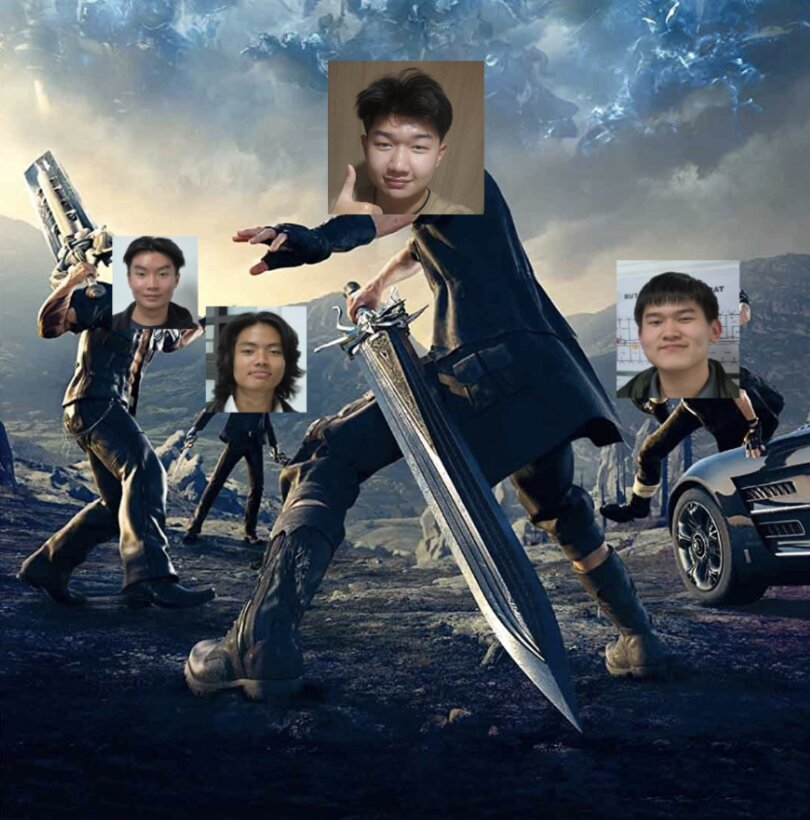
\includegraphics[width=0.55\textwidth]{gambar/foto-kelompok.jpg}
%==============================================================================
\thispagestyle{empty}
\begin{center}

\vspace*{0.5cm}

{\Large\bfseries LAPORAN TUGAS BESAR\par}
\vspace{0.3cm}
{\Large\bfseries IF2224 Teori Bahasa Formal dan Automata\par}
\vspace{0.2cm}
{\large\bfseries Semester II 2025/2026\par}

\vspace{0.8cm}

{\Large\bfseries\itshape Arion Compiler Milestone 4\par}
\vspace{0.2cm}
{\Large\bfseries\itshape Intermediate Code and Interpreter\par}

\vspace{0.7cm}

% ----- FOTO KELOMPOK (menggantikan logo ITB) -----
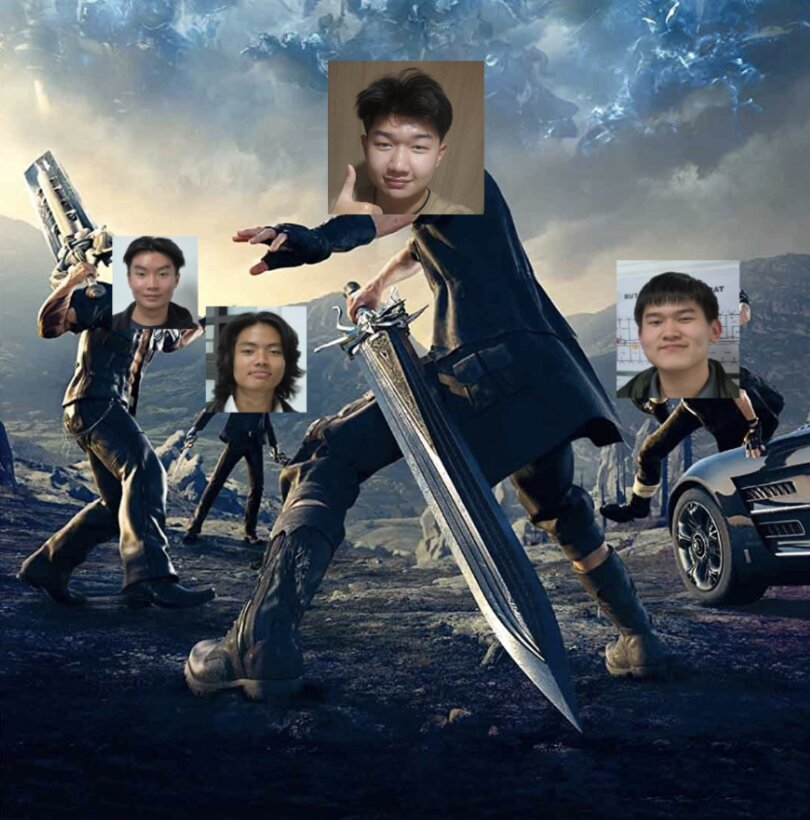
\includegraphics[width=0.50\textwidth]{gambar/foto-kelompok.jpg}

\vspace{0.7cm}

% ----- Anggota Kelompok -----
{\large
\renewcommand{\arraystretch}{1.4}
\begin{tabular}{l c}
Stevanus Agustaf Wongso & 13524020 \\
Renuno Yuqa Frinardi    & 13524080 \\
Valentino Daniel Kusumo & 13524104 \\
Michael James Liman     & 13524106 \\
\end{tabular}\par
}

\vfill

{\bfseries Sekolah Teknik Elektro dan Informatika\par}
{\bfseries Institut Teknologi Bandung\par}
{\bfseries 2026\par}

\vspace{0.5cm}
\end{center}


%---------------------------------------------------------------- Daftar isi
\newpage
\pagenumbering{roman}
\tableofcontents
\newpage
\pagenumbering{arabic}

%---------------------------------------------------------------- Isi laporan
%==============================================================================
%  BAB I - LANDASAN TEORI
%==============================================================================
\section{Landasan Teori}

Milestone 4 merupakan tahap akhir dari pengembangan kompiler bahasa Arion. Pada
tahap ini, \emph{Decorated AST} yang dihasilkan Milestone 3 diubah menjadi
\emph{Intermediate Code} berbentuk \emph{Three-Address Code} (TAC), lalu
dieksekusi oleh sebuah \emph{interpreter} berbasis \emph{stack machine} hingga
menghasilkan keluaran nyata program. Bab ini menjelaskan teori dan konsep yang
melandasi kedua komponen tersebut.

%------------------------------------------------------------------------------
\subsection{Arsitektur Kompiler: Front-end dan Back-end}

Kompiler modern umumnya dibagi menjadi dua fase arsitektur: \textbf{front-end}
dan \textbf{back-end}. Milestone 1 sampai 3 (analisis leksikal, sintaksis, dan
semantik) merupakan bagian front-end yang berurusan langsung dengan teks kode
sumber---memotongnya menjadi token, memvalidasi tata bahasanya, lalu memastikan
maknanya benar. Keluaran front-end adalah struktur data murni berupa
\emph{Decorated AST} yang sudah bebas dari teks mentah.

Milestone 4 sepenuhnya berada pada area back-end. Fase ini tidak lagi peduli
pada detail sintaksis Arion (titik koma, kurung, atau spasi), melainkan berfokus
pada dua tugas inti: \textbf{sintesis}, yaitu mengonversi Decorated AST menjadi
instruksi operasional standar (Intermediate Code), dan \textbf{eksekusi}, yaitu
mengelola memori serta menjalankan instruksi tersebut pada mesin virtual. Pemisahan
yang tegas ini memberi keuntungan rekayasa: bila suatu saat sintaks Arion diubah,
cukup front-end yang dirombak selama Decorated AST yang dihasilkan tetap sama,
back-end tidak perlu disentuh.

\begin{figure}[H]
\centering
\begin{tikzpicture}[
  node distance=0.55cm and 0.9cm,
  kotak/.style={draw, rounded corners, minimum height=1cm, minimum width=2.3cm,
    align=center, font=\footnotesize, fill=biruITB!8},
  kotakBE/.style={draw, rounded corners, minimum height=1cm, minimum width=2.3cm,
    align=center, font=\footnotesize, fill=hijauJudul!12},
  panah/.style={-{Stealth[length=2.5mm]}, thick}
]
  \node[kotak] (src) {Source\\Code};
  \node[kotak, right=of src] (tok) {Tokens};
  \node[kotak, right=of tok] (pt) {Parse\\Tree};
  \node[kotak, right=of pt] (ast) {Decorated\\AST};
  \node[kotakBE, below=1.1cm of ast] (tac) {Intermediate\\Code (TAC)};
  \node[kotakBE, left=of tac] (vm) {Stack\\Machine};
  \node[kotakBE, left=of vm] (out) {Program\\Output};

  \draw[panah] (src) -- (tok);
  \draw[panah] (tok) -- (pt);
  \draw[panah] (pt) -- (ast);
  \draw[panah] (ast) -- (tac);
  \draw[panah] (tac) -- (vm);
  \draw[panah] (vm) -- (out);

  \node[font=\scriptsize\itshape, above=0.05cm of tok] {Front-end (M1--M3)};
  \node[font=\scriptsize\itshape, below=0.05cm of vm] {Back-end (M4)};
\end{tikzpicture}
\caption{Pipeline kompiler Arion. Milestone 4 menambahkan tahap pembentukan
Intermediate Code dan eksekusi pada stack machine.}
\label{fig:pipeline}
\end{figure}

%------------------------------------------------------------------------------
\subsection{Intermediate Code Generation}

\subsubsection{Decorated AST sebagai Sumber Kebenaran}

\emph{Decorated AST} adalah \emph{Abstract Syntax Tree} yang setiap simpulnya
telah dianotasi (didekorasi) dengan informasi semantik, terutama \textbf{tipe
data} hasil ekspresi dan \textbf{referensi tabel simbol} untuk variabel. Anotasi
ini bersifat wajib bagi generator kode. Sebagai ilustrasi, ketika generator
menemui ekspresi \texttt{a + b}, tanpa informasi tipe ia tidak dapat memutuskan
apakah operasi tersebut penjumlahan bilangan atau penggabungan string. Dengan
Decorated AST, generator dapat memilih instruksi Intermediate Code yang tepat.

\subsubsection{Three-Address Code (TAC)}

Langkah berikutnya adalah meratakan (\emph{flattening}) Decorated AST menjadi
daftar instruksi linier. Format yang digunakan adalah \textbf{Three-Address
Code}, dinamai demikian karena tiap instruksi maksimal melibatkan tiga alamat
(dua operand sumber dan satu tujuan), dengan struktur dasar
\texttt{hasil = operand1 operator operand2}.

Karena CPU tidak dapat menghitung ekspresi panjang sekaligus, TAC memecah ekspresi
kompleks menggunakan \textbf{variabel sementara} (\emph{temporary}, ditulis
\texttt{t1}, \texttt{t2}, \dots). Pohon ekspresi dievaluasi dari cabang terdalam
menuju akar. Misalnya, ekspresi \texttt{x := (a + b) * (c - d)} diratakan menjadi:

\begin{lstlisting}[style=kodeTAC]
t1 := a + b      { evaluasi tanda kurung pertama }
t2 := c - d      { evaluasi tanda kurung kedua   }
t3 := t1 * t2    { kalikan hasil keduanya        }
x  := t3         { simpan hasil akhir ke x       }
\end{lstlisting}

Pada implementasi berbasis stack machine, peran variabel sementara digantikan oleh
puncak stack: hasil antara cukup ditinggalkan di atas stack untuk dikonsumsi
operasi berikutnya, sehingga tidak perlu dialokasikan nama \texttt{t1}, \texttt{t2}
secara eksplisit.

\subsubsection{Translasi Control Flow}

Tantangan terbesar pada pembentukan Intermediate Code adalah meratakan struktur
\emph{control flow} bersarang (\texttt{if-else}, \texttt{while}) menjadi daftar
linier. Solusinya menggunakan kombinasi \textbf{Label} dan \textbf{Jump}:

\textbf{Label} adalah penanda statis posisi suatu baris dalam TAC.
\textbf{Jump mutlak} (\texttt{JMP}) melompat tanpa syarat ke sebuah label,
sedangkan \textbf{jump bersyarat} (\texttt{JPC}) melompat hanya jika kondisi yang
dievaluasi bernilai \emph{false}. Konvensi melompat-jika-salah ini disebut
\emph{IF\_FALSE} dan memanfaatkan prinsip \emph{fall-through}: ketika kondisi
benar, eksekusi langsung berlanjut ke instruksi berikutnya tanpa lompatan,
sehingga alur kontrol menjadi lebih sederhana. Pada tugas besar ini konvensi
\emph{IF\_FALSE} bersifat wajib.

Berikut pola translasi \texttt{if-else} (kiri) dan \texttt{while} (kanan) menjadi
Intermediate Code.

\begin{center}
\begin{minipage}[t]{0.46\textwidth}
\centering\textbf{IF-ELSE}
\begin{lstlisting}[style=kodeTAC, numbers=none]
  t1 := x > 10
  JPC t1 -> L_ELSE
  y := 1
  JMP L_END
L_ELSE:
  y := 0
L_END:
\end{lstlisting}
\end{minipage}\hfill
\begin{minipage}[t]{0.46\textwidth}
\centering\textbf{WHILE}
\begin{lstlisting}[style=kodeTAC, numbers=none]
L_START:
  t1 := i < 5
  JPC t1 -> L_END
  i := i + 1
  JMP L_START
L_END:
\end{lstlisting}
\end{minipage}
\end{center}

%------------------------------------------------------------------------------
\subsection{Katalog Instruksi Intermediate Code}

Intermediate Code Arion menggunakan himpunan instruksi bergaya ORKOM. Tiap
instruksi terdiri atas \emph{mnemonic} dan operand opsional. Tabel~\ref{tab:instr}
merangkum instruksi yang didukung, sedangkan Tabel~\ref{tab:opr} merinci operasi
yang dipanggil melalui instruksi \texttt{OPR}.

\begin{table}[H]
\centering
\caption{Daftar instruksi Intermediate Code.}
\label{tab:instr}
\renewcommand{\arraystretch}{1.15}
\begin{tabularx}{\textwidth}{@{}l l X@{}}
\toprule
\textbf{Instruksi} & \textbf{Operasi} & \textbf{Keterangan} \\
\midrule
\texttt{LIT v} & Load Literal     & Memasukkan nilai literal \texttt{v} ke stack. \\
\texttt{LOD a} & Load Value       & Memuat nilai dari alamat \texttt{a} ke stack. \\
\texttt{STO a} & Store Value      & Mengambil nilai puncak stack, menyimpannya ke alamat \texttt{a}. \\
\texttt{CAL l} & Call             & Memanggil fungsi/prosedur pada baris \texttt{l}. \\
\texttt{INT m} & Initiate Memory  & Mengalokasikan memori (stack frame) berukuran \texttt{m}. \\
\texttt{JMP l} & Unconditional Jump & Lompat ke baris \texttt{l} tanpa syarat. \\
\texttt{JPC l} & Conditional Jump & Lompat ke baris \texttt{l} bila kondisi puncak stack salah. \\
\texttt{OPR o} & Operation        & Menjalankan operasi bernomor \texttt{o} (lihat Tabel~\ref{tab:opr}). \\
\texttt{RET}   & Return           & Keluar dari fungsi/prosedur atau mengakhiri program. \\
\bottomrule
\end{tabularx}
\end{table}

\begin{table}[H]
\centering
\caption{Daftar operasi instruksi \texttt{OPR}.}
\label{tab:opr}
\renewcommand{\arraystretch}{1.1}
\small
\begin{tabularx}{\textwidth}{@{}c l X | c l X@{}}
\toprule
\textbf{No} & \textbf{Nama} & \textbf{Fungsi} & \textbf{No} & \textbf{Nama} & \textbf{Fungsi} \\
\midrule
1 & NEG & Negasi puncak stack          & 8  & NEQ   & Tidak sama dengan \\
2 & ADD & Penjumlahan                  & 9  & LSS   & Kurang dari \\
3 & SUB & Pengurangan                  & 10 & GEQ   & Lebih dari sama dengan \\
4 & MUL & Perkalian                    & 11 & GTR   & Lebih dari \\
5 & DIV & Pembagian                    & 12 & LEQ   & Kurang dari sama dengan \\
6 & MOD & Modulus                      & 13 & WRT   & Cetak output \\
7 & EQL & Sama dengan                  & 14 & WRTLN & Cetak output + newline \\
\bottomrule
\end{tabularx}
\end{table}

%------------------------------------------------------------------------------
\subsection{Arsitektur Mesin Eksekusi: Interpreter dan Stack}

\subsubsection{Virtual Machine dan Siklus Eksekusi}

\emph{Interpreter} pada Milestone 4 berperan sebagai sebuah \emph{Virtual Machine}
(VM). Sama seperti CPU sungguhan, VM membaca instruksi satu per satu menggunakan
penunjuk \emph{Instruction Pointer} (IP) atau \emph{Program Counter}. VM bekerja
dalam \textbf{siklus eksekusi} tiga tahap: \textbf{Fetch} (membaca instruksi yang
ditunjuk IP), \textbf{Decode} (membedah mnemonic dan operand-nya), dan
\textbf{Execute} (melakukan aksi nyata). Setelah Execute, IP bergerak maju ke
instruksi berikutnya, kecuali pada instruksi lompat (\texttt{JMP}/\texttt{JPC})
yang menggeser IP langsung ke baris tujuan. Siklus berulang hingga IP mencapai
akhir program atau menemui \texttt{RET}.

\subsubsection{Memori Eksekusi: The Stack}

Struktur memori utama VM adalah \textbf{stack} yang bekerja dengan prinsip
\textbf{LIFO} (\emph{Last In, First Out})---data hanya bisa dimasukkan
(\emph{push}) dan diambil (\emph{pop}) dari puncak. Stack dipilih, bukan array
biasa, karena berkaitan erat dengan \emph{scope} dan pemanggilan fungsi. Setiap
kali program memasuki blok atau memanggil fungsi, VM membuat \emph{stack frame}
baru. Pada konvensi yang dipakai, tiga sel pertama setiap frame selalu terisi
\textbf{Static Link} (alamat 0), \textbf{Dynamic Link} (alamat 1), dan
\textbf{Return Address} (alamat 2); sel selanjutnya (mulai alamat 3) digunakan
untuk variabel. Akses variabel dilakukan relatif terhadap \emph{Base Pointer}
(BP) frame aktif, sementara \emph{Stack Pointer} (SP) menunjuk puncak stack.

\begin{figure}[H]
\centering
\begin{tikzpicture}[
  sel/.style={draw, minimum width=5.5cm, minimum height=0.7cm, font=\footnotesize, anchor=south west},
  selV/.style={sel, fill=hijauJudul!12},
  selR/.style={sel, fill=biruITB!10},
]
  \node[selR] at (0,0)   (a0) {alamat 0 -- Static Link};
  \node[selR] at (0,0.7) (a1) {alamat 1 -- Dynamic Link};
  \node[selR] at (0,1.4) (a2) {alamat 2 -- Return Address};
  \node[selV] at (0,2.1) (a3) {alamat 3 -- Variable (x)};
  \node[selV] at (0,2.8) (a4) {alamat 4 -- Variable (y)};
  \node[sel, fill=white] at (0,3.5) (a5) {puncak -- operand/hasil sementara};

  \node[font=\footnotesize, right=0.3cm of a0] {$\leftarrow$ BP (basis frame)};
  \node[font=\footnotesize, right=0.3cm of a5] {$\leftarrow$ SP (puncak stack)};
\end{tikzpicture}
\caption{Struktur stack frame: tiga sel administratif diikuti sel variabel; ruang
di atasnya dipakai sebagai operand dan hasil sementara perhitungan.}
\label{fig:frame}
\end{figure}

%------------------------------------------------------------------------------
\subsection{Keamanan Runtime dan Penanganan Kerentanan}

Interpreter yang tangguh tidak hanya menjalankan kode yang benar, tetapi juga
mampu bertahan (tidak \emph{crash}) ketika diberi kode yang salah atau tidak
masuk akal. Berbeda dengan bahasa tingkat rendah yang menyerahkan keamanan kepada
\emph{programmer}, bahasa yang berjalan di atas VM wajib memiliki mekanisme
perlindungan internal. Sebagai bagian dari spesifikasi (termasuk tantangan bonus),
interpreter Arion mendeteksi dan menangani sejumlah kerentanan berikut.

\textbf{Kerentanan pada stack.} \emph{Stack overflow} terjadi ketika frame terus
ditambahkan melampaui batas memori, umumnya akibat rekursi tanpa \emph{base case};
interpreter membatasi kedalaman frame dan melempar error bila terlampaui.
\emph{Stack underflow} terjadi ketika operasi \emph{pop} dipanggil saat stack
kosong. \emph{Stack smashing} adalah perusakan \emph{return address} oleh data yang
meluber, dideteksi menggunakan \emph{canary} pada sel return address.
\emph{Stack corruption} terjadi ketika jumlah \emph{push} dan \emph{pop} tidak
simetris sehingga indeks frame bergeser; ini dideteksi dengan memverifikasi posisi
stack pointer saat keluar dari frame.

\textbf{Kerentanan memori dan alur.} \emph{Out-of-Bounds Access} dicegah dengan
memvalidasi setiap alamat pada \texttt{LOD}/\texttt{STO} terhadap batas memori.
\emph{Invalid Jump Target} dicegah dengan memverifikasi target \texttt{JMP},
\texttt{JPC}, dan \texttt{CAL} berada dalam rentang program sebelum IP dipindahkan.

\textbf{Kerentanan aritmatika.} Tipe \emph{integer} memiliki kapasitas terbatas;
operasi yang melampaui batas atas (\emph{overflow}) atau bawah (\emph{underflow})
akan menyebabkan \emph{wrap-around} yang mengacaukan perhitungan. Interpreter
mendeteksi kondisi ini sebelum hasil sempat membungkus, lalu melempar
\textbf{OverflowError} atau \textbf{UnderflowError}. Demikian pula pembagian dengan
nol dicegat sebagai \textbf{DivisionByZeroError}.

\textbf{Runtime type checking.} Karena Arion bersifat \emph{strongly-typed} dan
sebagian besar tipe telah diverifikasi pada analisis semantik, runtime type
checking tidak diwajibkan. Meski demikian, interpreter tetap memvalidasi bahwa
operand operasi aritmatika benar-benar bernilai numerik saat eksekusi; bila tidak,
ia melempar \textbf{TypeMismatchError} alih-alih melakukan konversi diam-diam.

%==============================================================================
%  BAB II - PERANCANGAN DAN IMPLEMENTASI
%==============================================================================
\section{Perancangan dan Implementasi}

%==============================================================================
\subsection{Perancangan}

\subsubsection{Gambaran Umum Sistem}

Pada Milestone 4, program menambahkan dua tahap baru pada pipeline kompiler:
\emph{Intermediate Code Generation} dan \emph{Execution}. Alur kerjanya dapat
diringkas sebagai berikut.

\begin{center}
\fcolorbox{abuGaris}{abuKode}{\parbox{0.92\textwidth}{\centering\ttfamily
Decorated AST $\rightarrow$ Intermediate Code (TAC) $\rightarrow$ Stack Machine $\rightarrow$ Program Output}}
\end{center}

Generator menerima Decorated AST hasil Milestone 3 lalu menelusurinya untuk
menghasilkan daftar instruksi TAC. Daftar tersebut kemudian dikonversi melalui
sebuah \emph{adapter} dan dieksekusi oleh stack machine, yang mengelola memori
dalam bentuk stack dan mencetak keluaran nyata ketika menemui instruksi
\texttt{WRT}/\texttt{WRTLN}. Spesifikasi prosesnya: \textbf{masukan} berupa
Decorated AST, \textbf{keluaran} berupa Intermediate Code beserta output program,
dengan \textbf{algoritma} penelusuran berbasis DFS untuk pembentukan TAC dan
\emph{stack machine} untuk eksekusi.

\subsubsection{Teknologi yang Digunakan}

Sesuai ketentuan, bahasa pemrograman yang digunakan disamakan dengan milestone
sebelumnya, yaitu \textbf{C++} dengan standar \textbf{C++17}, dikompilasi
menggunakan \texttt{g++} dan diotomasi dengan \textbf{GNU Make}. Tidak ada
pustaka eksternal yang digunakan; seluruh komponen dibangun di atas pustaka
standar C++ (\texttt{<vector>}, \texttt{<string>}, \texttt{<unordered\_map>},
\texttt{<sstream>}, \texttt{<memory>}). Deteksi \emph{overflow} aritmatika
memanfaatkan \emph{builtin} \texttt{\_\_builtin\_*\_overflow} milik \texttt{g++}.

\subsubsection{Struktur Modul dan Arsitektur File}

Sesuai prinsip modularitas, kode Milestone 4 dipisahkan berdasarkan tanggung
jawab ke dalam dua direktori: \texttt{src/intermediate/} (pembentukan TAC) dan
\texttt{src/interpreter/} (eksekusi). Tabel~\ref{tab:file} memerinci berkas-berkas
baru beserta perannya.

\begin{table}[H]
\centering
\caption{Arsitektur berkas Milestone 4.}
\label{tab:file}
\renewcommand{\arraystretch}{1.2}
\begin{tabularx}{\textwidth}{@{}l X@{}}
\toprule
\textbf{Berkas} & \textbf{Tanggung Jawab} \\
\midrule
\texttt{intermediate/tac.\{hpp,cpp\}}     & Kelas \texttt{TacGenerator}: konversi Decorated AST $\rightarrow$ TAC. \\
\texttt{interpreter/runtime\_value.*}      & Struktur \texttt{RuntimeValue}: nilai bertipe pada stack. \\
\texttt{interpreter/runtime\_instruction.hpp} & Struktur \texttt{RuntimeInstruction}: satu instruksi siap eksekusi. \\
\texttt{interpreter/runtime\_context.*}    & Struktur \texttt{RuntimeContext}: stack, IP, BP, dan pembukuan frame. \\
\texttt{interpreter/stack\_machine.*}      & Kelas \texttt{StackMachine}: inti siklus fetch--decode--execute. \\
\texttt{interpreter/runtime\_error\_hook.*}& \texttt{RuntimeErrorHook}: klasifikasi dan pelemparan error runtime. \\
\texttt{interpreter/tac\_adapter.*}        & \texttt{TacAdapter}: jembatan \texttt{TacInstr} $\rightarrow$ \texttt{RuntimeInstruction}. \\
\texttt{interpreter/interpreter.*}         & Kelas \texttt{Interpreter}: pembungkus VM + penangkap error. \\
\bottomrule
\end{tabularx}
\end{table}

\subsubsection{Justifikasi Pilihan Implementasi}

\textbf{Penelusuran berbasis DFS.} Pembentukan TAC dilakukan dengan menelusuri AST
secara \emph{depth-first}. Untuk ekspresi, penelusuran postorder menjamin operand
sudah berada di stack sebelum operatornya dijalankan; untuk pernyataan,
penelusuran preorder yang dipadu pembentukan label menjaga urutan eksekusi sesuai
struktur program.

\textbf{Stack machine, bukan register machine.} Model stack machine dipilih karena
selaras dengan konvensi instruksi yang disediakan (gaya ORKOM) dan menghapus
kebutuhan akan alokasi register/variabel sementara eksplisit---hasil antara cukup
ditinggalkan pada puncak stack.

\textbf{Pola Adapter.} \texttt{TacGenerator} (tim pembentuk kode) dan
\texttt{StackMachine} (tim interpreter) sengaja dipisahkan oleh
\texttt{TacAdapter}. Dengan begitu, kode interpreter tidak bergantung pada detail
internal generator; perubahan pada salah satu sisi tidak merembet ke sisi lain.

\textbf{Error sebagai pengecualian, bukan crash.} Seluruh pelanggaran runtime
dilempar sebagai \texttt{RuntimeError} dan ditangkap di satu titik
(\texttt{Interpreter::run}), sehingga program selalu berhenti secara \emph{graceful}
dengan pesan informatif alih-alih \emph{segmentation fault}.

%==============================================================================
\subsection{Implementasi Intermediate Code Generator}

\texttt{TacGenerator} mengubah Decorated AST menjadi vektor \texttt{TacInstr}.
Tiap instruksi merekam \emph{opcode}, daftar argumen, label opsional, serta target
lompat yang terisi setelah resolusi.

\subsubsection{Pemetaan Alamat Memori}

Sebelum kode dihasilkan, seluruh deklarasi variabel dipindai dan dipetakan ke
alamat memori mulai dari 3 (sel 0--2 dicadangkan untuk static link, dynamic link,
dan return address). Ukuran memori frame utama lalu dialokasikan dengan instruksi
\texttt{INT} sebesar $3 + (\text{jumlah variabel})$.

\begin{lstlisting}[style=kodeCpp, caption={Pemetaan alamat variabel dan alokasi memori awal.}]
void TacGenerator::collectDecls(const AstNodePtr& program) {
    for (auto& child : program->children) {
        if (child->kind != AstKind::Declarations) continue;
        for (auto& decl : child->children) {
            if (decl->kind == AstKind::VarDecl && !decl->value.empty()) {
                string key = lower(decl->value);
                if (addrMap.find(key) == addrMap.end())
                    addrMap[key] = nextAddr++;   // 3, 4, 5, ...
            }
        }
    }
}
// ... pada generate():
int varCount = static_cast<int>(addrMap.size());
emit("INT", {"0", to_string(3 + varCount)});     // INT 0 <3 + jml var>
\end{lstlisting}

\subsubsection{Pembentukan Ekspresi (DFS Postorder)}

Ekspresi dibentuk secara rekursif. Literal menjadi \texttt{LIT}, variabel menjadi
\texttt{LOD} pada alamatnya, sedangkan operasi biner mem-\emph{push} operand kiri
lalu kanan sebelum memanggil \texttt{OPR} dengan opcode yang sesuai. Pemetaan
operator ke opcode mengikuti Tabel~\ref{tab:opr}.

\begin{lstlisting}[style=kodeCpp, caption={Pembentukan ekspresi: hasil ditinggalkan di puncak stack.}]
void TacGenerator::genExpr(const AstNodePtr& node) {
    switch (node->kind) {
        case AstKind::Number: case AstKind::RealNumber:
        case AstKind::BoolLit: /* ... */
            emit("LIT", {"0", node->value});               break;
        case AstKind::Var:
            emit("LOD", {"0", to_string(addrOf(node))});   break;
        case AstKind::BinOp: {
            genExpr(node->children[0]);   // operand kiri di-push lebih dulu
            genExpr(node->children[1]);   // lalu operand kanan
            int code = oprCode(node->value);
            if (code >= 0) emit("OPR", {"0", to_string(code)});
            break;
        }
        case AstKind::UnaryOp:
            genExpr(node->children[0]);
            if (node->value == "-") emit("OPR", {"0", "1"});  // NEG
            break;
    }
}
\end{lstlisting}

\subsubsection{Pembentukan Control Flow}

Pernyataan \texttt{if} dan \texttt{while} dibentuk dengan menyemai label simbolik
(\texttt{L1}, \texttt{L2}, \dots) yang nantinya diresolusi menjadi nomor baris.
Konvensi \emph{IF\_FALSE} diwujudkan oleh \texttt{JPC}: kondisi di-\emph{push},
lalu \texttt{JPC} melompati blok bila kondisi salah.

\begin{lstlisting}[style=kodeCpp, caption={Pembentukan \texttt{if-else} dan \texttt{while} dengan label \& jump.}]
void TacGenerator::genIf(const AstNodePtr& node) {
    string elseLbl = newLabel(), endLbl = newLabel();
    genExpr(cond);                    // push kondisi
    emit("JPC", {"0", elseLbl});      // salah -> lompat ke else
    if (thenNode) genNode(thenNode);
    if (elseNode) emit("JMP", {"0", endLbl});
    emitLabel(elseLbl);
    if (elseNode) genNode(elseNode);
    emitLabel(endLbl);
}

void TacGenerator::genWhile(const AstNodePtr& node) {
    string startLbl = newLabel(), endLbl = newLabel();
    emitLabel(startLbl);
    genExpr(cond);                    // push kondisi
    emit("JPC", {"0", endLbl});       // salah -> keluar loop
    if (body) genNode(body);
    emit("JMP", {"0", startLbl});     // ulangi
    emitLabel(endLbl);
}
\end{lstlisting}

\subsubsection{Resolusi Label dan Pencetakan}

Setelah seluruh kode terbentuk, label diresolusi menjadi nomor baris 1-\emph{based},
lalu \emph{pseudo-op} \texttt{LABEL} dihapus agar daftar instruksi padat dan langsung
dapat dieksekusi (jika dibiarkan, label akan menggeser indeks setiap instruksi
sesudahnya). Saat dicetak, \texttt{JMP}/\texttt{JPC} ditampilkan dengan target
numeriknya dalam format kanonik \texttt{<baris> <OP> <lev> <operand>}.

%==============================================================================
\subsection{Implementasi Interpreter (Stack Machine)}

\subsubsection{Representasi Nilai dan Konteks}

Setiap sel stack menyimpan \texttt{RuntimeValue} yang bertipe (\texttt{INTEGER},
\texttt{REAL}, \texttt{BOOLEAN}, \texttt{CHAR}, \texttt{STRING}, atau
\texttt{NONE}). Tipe yang melekat inilah yang memungkinkan \emph{runtime type
checking} dan pencetakan keluaran yang benar. Seluruh keadaan eksekusi disimpan
dalam \texttt{RuntimeContext}: vektor \texttt{stack}, base pointer \texttt{bp},
return address \texttt{ra}, dynamic link \texttt{dl}, kedalaman frame, instruction
pointer \texttt{ip}, vektor program, serta \emph{buffer} keluaran.

\subsubsection{Siklus Fetch--Decode--Execute}

Metode \texttt{run()} mengulang \texttt{step()} hingga program \emph{halt} atau IP
melewati akhir program. Tiap \texttt{step()} membaca instruksi pada IP lalu
mendispatch ke \emph{handler} sesuai opcode.

\begin{lstlisting}[style=kodeCpp, caption={Inti siklus eksekusi dan dispatch instruksi.}]
void StackMachine::run() {
    while (!context.halted && context.ip < context.program.size())
        step();
}
void StackMachine::execute(const RuntimeInstruction& instr) {
    const string& op = instr.op;
    if (op == "INT") { execINT(instr); return; }
    if (op == "LIT") { execLIT(instr); return; }
    if (op == "LOD") { execLOD(instr); return; }
    if (op == "STO") { execSTO(instr); return; }
    if (op == "JMP") { execJMP(instr); return; }
    if (op == "JPC") { execJPC(instr); return; }
    if (op == "OPR") { execOPR(instr); return; }
    if (op == "RET") { execRET(instr); return; }
    // ... CAL, LABEL ...
    RuntimeErrorHook::invalidOperand(op, "unknown instruction");
}
\end{lstlisting}

\subsubsection{Inisiasi Frame dan Akses Memori}

Instruksi \texttt{INT} membentuk frame baru: mendorong static link, dynamic link,
dan return address, lalu mengalokasikan sel variabel. Akses variabel
(\texttt{LOD}/\texttt{STO}) dihitung relatif terhadap \texttt{bp} dan divalidasi
terhadap batas stack sebelum digunakan.

\begin{lstlisting}[style=kodeCpp, caption={\texttt{LOD} dengan validasi akses memori (mencegah OOB).}]
void StackMachine::execLOD(const RuntimeInstruction& instr) {
    int addr = parseIntArg(instr, 1);
    int absIdx = context.bp + addr;
    if (absIdx < 0 || (size_t)absIdx >= context.stack.size())
        RuntimeErrorHook::invalidMemoryAccess(addr, context.bp,
                                              context.stack.size());
    push(context.stack[absIdx]);
    context.ip++;
}
\end{lstlisting}

\subsubsection{Lompatan dan Konvensi IF\_FALSE}

\texttt{JPC} mengeluarkan kondisi dari puncak stack; bila bernilai \emph{false}, IP
dipindahkan ke target, jika tidak IP maju satu langkah. Setiap target lompat
divalidasi oleh \texttt{resolveJump} agar tidak menunjuk ke luar program.

\begin{lstlisting}[style=kodeCpp, caption={\texttt{JPC} (jump-if-false) dan validasi target lompat.}]
void StackMachine::execJPC(const RuntimeInstruction& instr) {
    RuntimeValue cond = pop();
    if (!cond.isTruthy()) context.ip = resolveJump(instr.target);
    else                  context.ip++;
}
size_t StackMachine::resolveJump(int target) const {
    int n = (int)context.program.size();
    if (target < 1 || target > n)
        RuntimeErrorHook::invalidJumpTarget(target, n);
    return (size_t)(target - 1);   // 1-based -> 0-based
}
\end{lstlisting}

\subsubsection{Operasi melalui OPR}

\texttt{execOPR} mendispatch nomor operasi ke sub-handler. Operasi aritmatika
mengeluarkan dua operand (atau satu untuk \texttt{NEG}), memvalidasi tipenya,
melakukan perhitungan ber-\emph{checked} terhadap overflow, lalu mem-\emph{push}
hasilnya. Operasi perbandingan menghasilkan \texttt{BOOLEAN}, sedangkan
\texttt{WRT}/\texttt{WRTLN} menulis nilai puncak stack ke \emph{buffer} keluaran.

%==============================================================================
\subsection{Implementasi Error Handling dan Keamanan Runtime}

Seluruh kondisi error dipusatkan pada modul \texttt{RuntimeErrorHook}. Setiap
pelanggaran memanggil fungsi yang memformat pesan \texttt{[ERROR] <Jenis>: <detail> !}
lalu melempar \texttt{RuntimeError} dengan klasifikasi jenisnya, sehingga pesan
konsisten dan mudah ditelusuri.

\textbf{Aritmatika ber-checked.} Operasi integer memakai \emph{builtin} g++ untuk
mendeteksi \emph{wrap-around}, lalu melempar \texttt{OverflowError}/\texttt{UnderflowError}.

\begin{lstlisting}[style=kodeCpp, caption={Penjumlahan dengan deteksi overflow/underflow.}]
long long StackMachine::addChecked(long long a, long long b, const string& op) {
    long long r;
    if (__builtin_add_overflow(a, b, &r)) {
        if (a > 0 && b > 0) RuntimeErrorHook::numericOverflow(op);
        RuntimeErrorHook::numericUnderflow(op);
    }
    return r;
}
\end{lstlisting}

\textbf{Deteksi stack corruption dan smashing.} Saat \texttt{INT}, sebuah
\texttt{FrameGuard} mencatat posisi puncak yang seharusnya saat keluar
(\emph{expected top}) dan salinan return address sebagai \emph{canary}. Pada
\texttt{RET}, posisi puncak aktual dibandingkan dengan \emph{expected top} (deteksi
\emph{corruption}) dan sel return address dibandingkan dengan \emph{canary}
(deteksi \emph{smashing}).

\begin{lstlisting}[style=kodeCpp, caption={Verifikasi keseimbangan frame saat \texttt{RET}.}]
const FrameGuard guard = context.frames.back();
context.frames.pop_back();
int actualTop = (int)context.stack.size();
if (actualTop != guard.expectedTop)              // push/pop tak simetris
    RuntimeErrorHook::stackCorruption("unbalanced push/pop ...",
                                      guard.expectedTop, actualTop);
int raIdx = guard.basePtr + 2;                    // sel return address
if (context.stack[raIdx].intVal != guard.canaryRa)
    RuntimeErrorHook::stackSmashing(guard.canaryRa, context.stack[raIdx].intVal);
\end{lstlisting}

Tabel~\ref{tab:err} merangkum jenis-jenis error runtime yang ditangani beserta
mekanisme deteksinya.

\begin{table}[H]
\centering
\caption{Ringkasan penanganan error runtime.}
\label{tab:err}
\renewcommand{\arraystretch}{1.15}
\begin{tabularx}{\textwidth}{@{}l X@{}}
\toprule
\textbf{Jenis Error} & \textbf{Mekanisme Deteksi} \\
\midrule
DivisionByZeroError      & Pembagi bernilai nol pada \texttt{DIV}/\texttt{MOD}. \\
OverflowError / UnderflowError & Hasil aritmatika integer membungkus (\emph{wrap-around}). \\
StackOverflowError       & Kedalaman frame atau ukuran stack melampaui batas. \\
StackUnderflowError      & \emph{Pop} dipanggil saat stack kekurangan nilai. \\
InvalidJumpError         & Target \texttt{JMP}/\texttt{JPC}/\texttt{CAL} di luar program. \\
InvalidMemoryAccessError & Alamat \texttt{LOD}/\texttt{STO} di luar batas stack. \\
StackCorruptionError     & Posisi stack pointer tidak sesuai saat keluar frame. \\
StackSmashingError       & \emph{Canary} return address tertimpa data lain. \\
TypeMismatchError        & Operand aritmatika ternyata bukan nilai numerik. \\
InvalidOperandError      & Argumen instruksi hilang atau bukan integer valid. \\
\bottomrule
\end{tabularx}
\end{table}

%==============================================================================
%  BAB III - PENGUJIAN
%==============================================================================
\section{Pengujian}

Bagian ini menyajikan enam kasus uji unik yang mencakup penugasan, ekspresi
aritmatika dan relasional, ekspresi bersarang, alur kontrol, serta dua kasus
penanganan error runtime. Setiap kasus menampilkan kode sumber Arion sebagai
masukan, Intermediate Code yang dihasilkan, dan keluaran nyata program. Seluruh
hasil di bawah diperoleh dengan menjalankan kompiler pada berkas uji yang
bersangkutan; bukti tangkapan layar disertakan sebagai placeholder.

%------------------------------------------------------------------------------
\subsection{Kasus 1 -- Penugasan dan Cetak Literal}

\textbf{Tujuan.} Memverifikasi alokasi memori (\texttt{INT}), penugasan literal ke
variabel (\texttt{LIT}+\texttt{STO}), pembacaan kembali (\texttt{LOD}), dan
penimpaan nilai variabel.

\begin{minipage}[t]{0.48\textwidth}
\textbf{Masukan} (\texttt{src\_assignment.txt}):
\begin{lstlisting}[style=kodeArion, numbers=none]
program SimpleAssign;
var
  n: integer;
begin
  n := 10;
  writeln(n);
  n := 99;
  writeln(n);
end.
\end{lstlisting}
\end{minipage}\hfill
\begin{minipage}[t]{0.48\textwidth}
\textbf{Intermediate Code:}
\begin{lstlisting}[style=kodeTAC, numbers=none]
1 INT 0 4
2 LIT 0 10
3 STO 0 3
4 LOD 0 3
5 OPR 0 14
6 LIT 0 99
7 STO 0 3
8 LOD 0 3
9 OPR 0 14
10 RET 0 0
\end{lstlisting}
\end{minipage}

\textbf{Keluaran Program:}
\begin{lstlisting}[style=kodeTAC, numbers=none]
10
99
\end{lstlisting}

\begin{center}
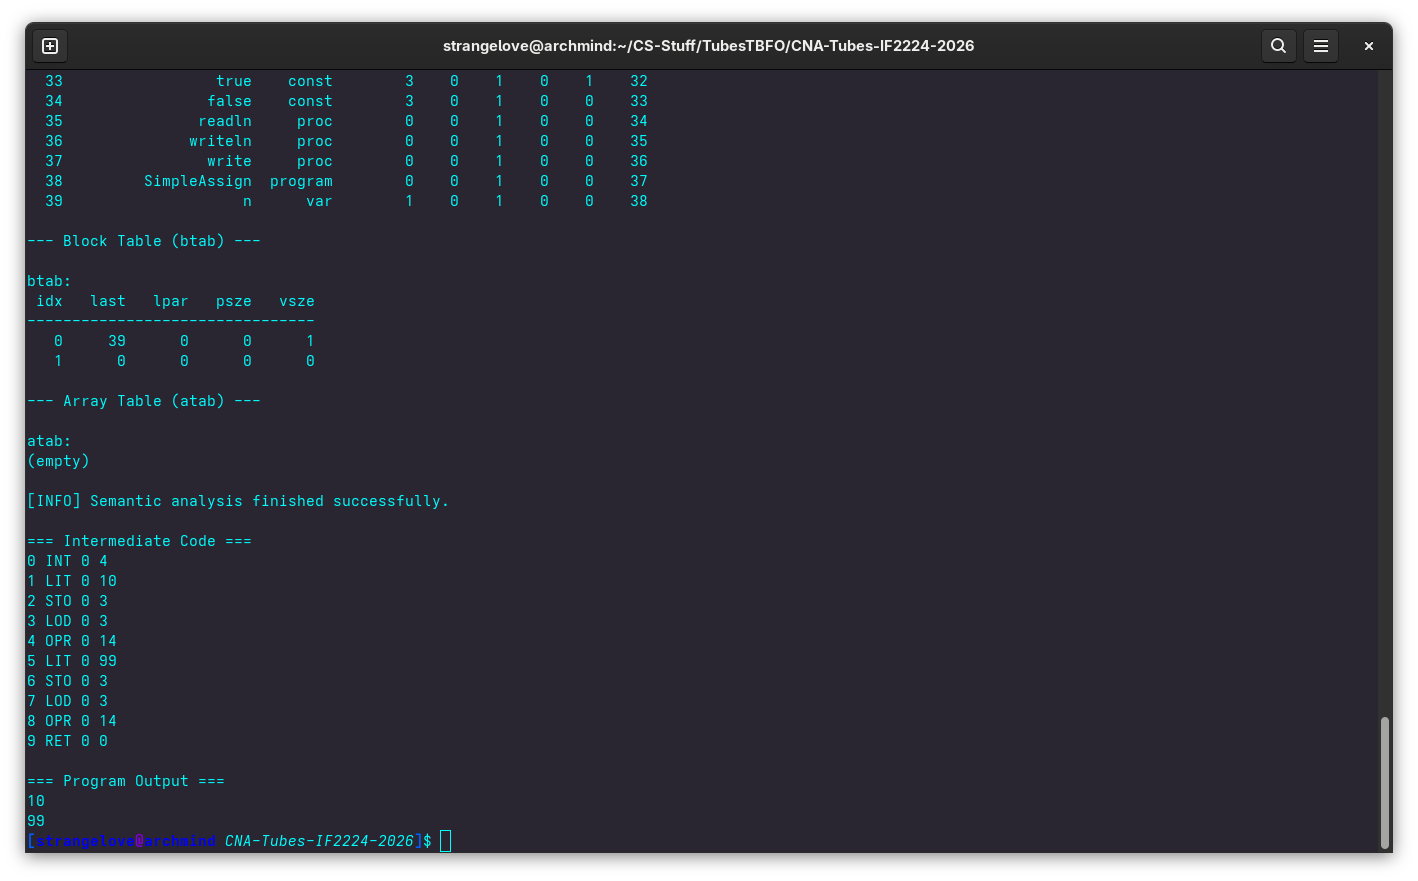
\includegraphics[width=14cm]{gambar/tc1_src_assignment.png}
\end{center}

\textbf{Analisis.} Variabel \texttt{n} dipetakan ke alamat 3 sehingga \texttt{INT}
mengalokasikan 4 sel (3 administratif + 1 variabel). Penimpaan \texttt{n := 99}
menyimpan ulang ke alamat yang sama. Keluaran sesuai harapan.

%------------------------------------------------------------------------------
\subsection{Kasus 2 -- Ekspresi Aritmatika dan Relasional}

\textbf{Tujuan.} Menguji operator aritmatika (\texttt{+}, \texttt{-}, \texttt{*},
\texttt{div}), prioritas tanda kurung, serta operator relasional yang menghasilkan
nilai \texttt{boolean}.

\begin{minipage}[t]{0.48\textwidth}
\textbf{Masukan} (\texttt{src\_expr\_assign.txt}):
\begin{lstlisting}[style=kodeArion, numbers=none]
program ExprAssign;
var
  a, b, c: integer;
begin
  a := 6 + 4;
  b := (a - 2) * 3;
  c := b div 5;
  writeln(a);
  writeln(b);
  writeln(c);
  writeln(a = 10);
  writeln(b > c);
end.
\end{lstlisting}
\end{minipage}\hfill
\begin{minipage}[t]{0.48\textwidth}
\textbf{Intermediate Code:}
\begin{lstlisting}[style=kodeTAC, numbers=none]
1 INT 0 6      16 LOD 0 3
2 LIT 0 6      17 OPR 0 14
3 LIT 0 4      18 LOD 0 4
4 OPR 0 2      19 OPR 0 14
5 STO 0 3      20 LOD 0 5
6 LOD 0 3      21 OPR 0 14
7 LIT 0 2      22 LOD 0 3
8 OPR 0 3      23 LIT 0 10
9 LIT 0 3      24 OPR 0 7
10 OPR 0 4     25 OPR 0 14
11 STO 0 4     26 LOD 0 4
12 LOD 0 4     27 LOD 0 5
13 LIT 0 5     28 OPR 0 11
14 OPR 0 5     29 OPR 0 14
15 STO 0 5     30 RET 0 0
\end{lstlisting}
\end{minipage}

\textbf{Keluaran Program:}
\begin{lstlisting}[style=kodeTAC, numbers=none]
10
24
4
TRUE
TRUE
\end{lstlisting}

\begin{center}
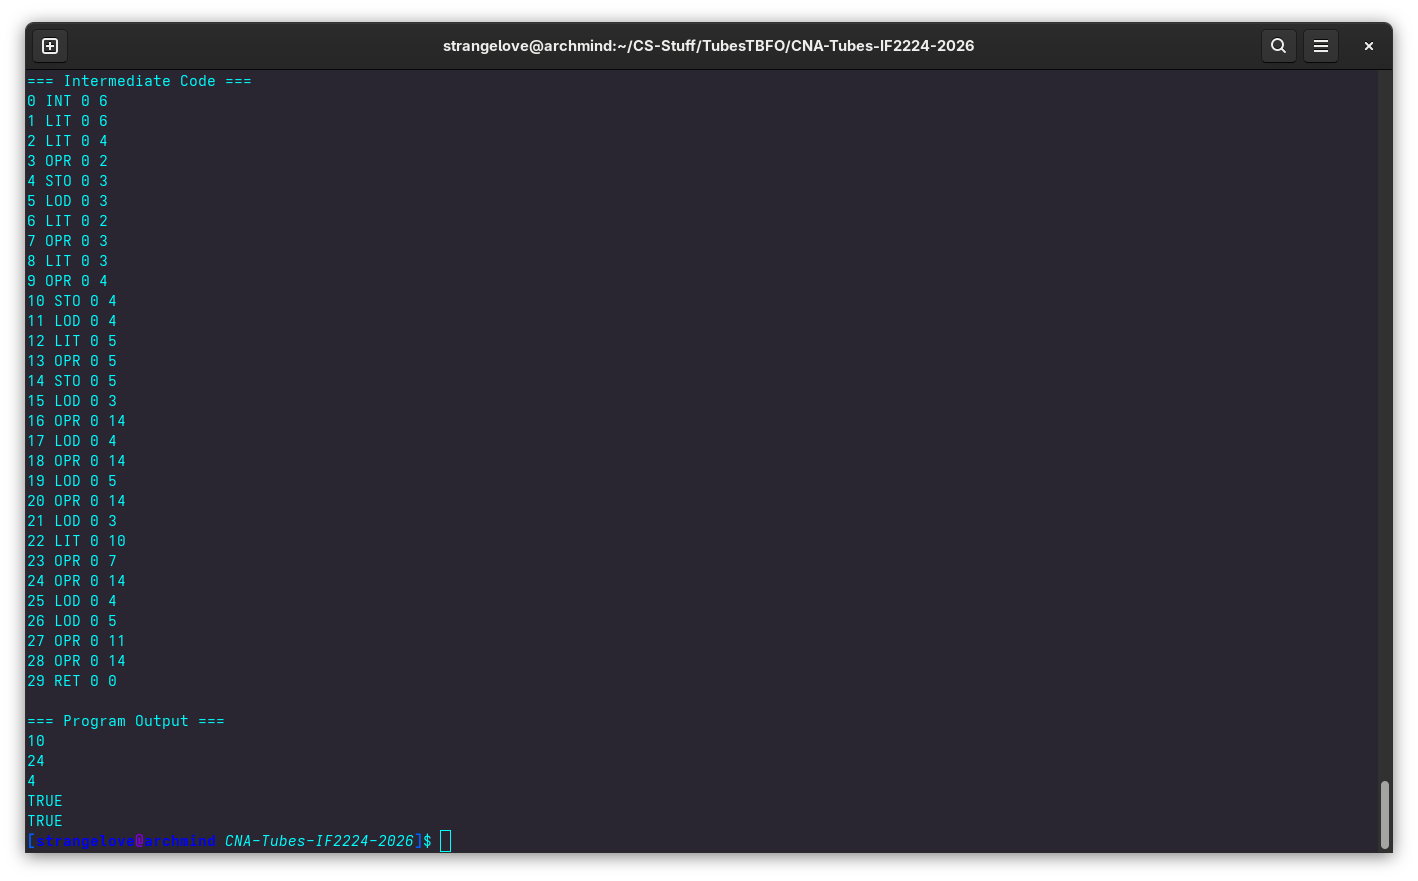
\includegraphics[width=15cm]{gambar/tc2_src_expr_assign.png}
\end{center}

\textbf{Analisis.} Perhitungan terverifikasi: $a = 10$, $b = (10-2)\times 3 = 24$,
$c = 24 \div 5 = 4$ (pembagian integer). Operator relasional \texttt{=} (OPR 7) dan
\texttt{>} (OPR 11) menghasilkan \texttt{boolean} yang dicetak sebagai
\texttt{TRUE}.

%------------------------------------------------------------------------------
\subsection{Kasus 3 -- Ekspresi Bersarang dan Modulus}

\textbf{Tujuan.} Memastikan penelusuran DFS meratakan ekspresi bersarang
\texttt{(a + b) * (c - d)} dengan benar---hasil antara ditinggalkan di puncak
stack sebagai pengganti variabel sementara---serta menguji operator \texttt{mod}.

\begin{minipage}[t]{0.48\textwidth}
\textbf{Masukan} (\texttt{src\_nested\_expr.txt}):
\begin{lstlisting}[style=kodeArion, numbers=none]
program NestedExpr;
var
  a, b, c, d, x: integer;
begin
  a := 3;  b := 4;
  c := 10; d := 2;
  x := (a + b) * (c - d);
  writeln(x);
  writeln(c mod d);
end.
\end{lstlisting}
\end{minipage}\hfill
\begin{minipage}[t]{0.48\textwidth}
\textbf{Intermediate Code (ringkas):}
\begin{lstlisting}[style=kodeTAC, numbers=none]
 1 INT 0 8     13 LOD 0 5
 2 LIT 0 3     14 LOD 0 6
 3 STO 0 3     15 OPR 0 3   ; c - d
 ...           16 OPR 0 4   ; (..)*(..)
10 LOD 0 3     17 STO 0 7
11 LOD 0 4     18 LOD 0 7
12 OPR 0 2     19 OPR 0 14  ; writeln(x)
 ; c - d       20 LOD 0 5
               21 LOD 0 6
               22 OPR 0 6   ; c mod d
               23 OPR 0 14
               24 RET 0 0
\end{lstlisting}
\end{minipage}

\textbf{Keluaran Program:}
\begin{lstlisting}[style=kodeTAC, numbers=none]
56
0
\end{lstlisting}

\begin{center}
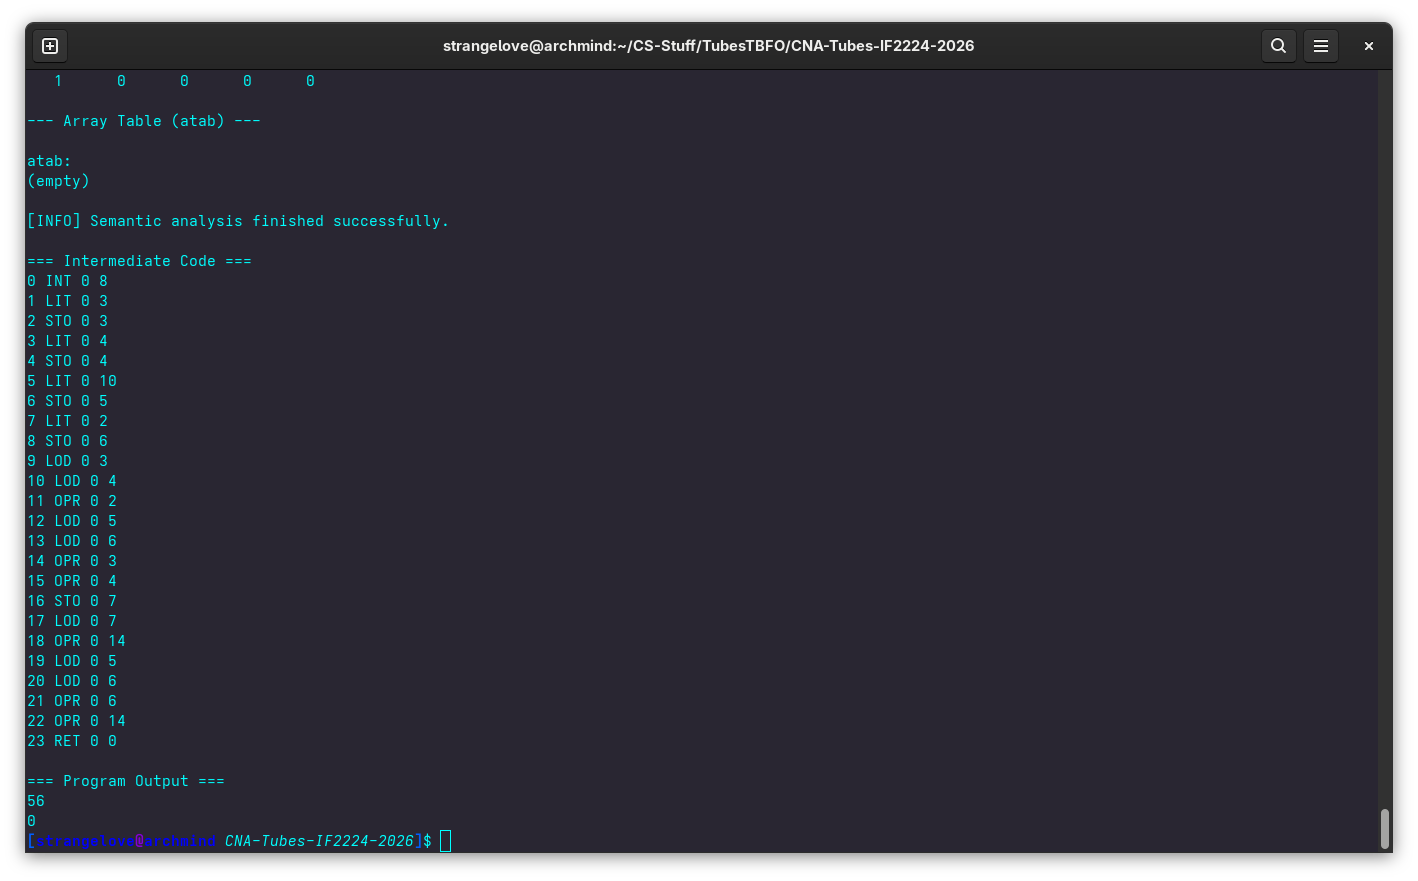
\includegraphics[width=15cm]{gambar/tc3_src_nested_expr.png}
\end{center}

\textbf{Analisis.} $x = (3+4)\times(10-2) = 7 \times 8 = 56$ dan
$c \bmod d = 10 \bmod 2 = 0$. Subekspresi kiri dihitung lebih dulu (OPR 2), lalu
subekspresi kanan (OPR 3), barulah keduanya dikalikan (OPR 4)---membuktikan urutan
evaluasi postorder yang benar tanpa membutuhkan nama \texttt{temporary} eksplisit.

%------------------------------------------------------------------------------
\subsection{Kasus 4 -- Kontrol Alur IF-ELSE dan WHILE}

\textbf{Tujuan.} Menguji translasi percabangan dan perulangan---konvensi
\emph{IF\_FALSE} pada \texttt{JPC}, lompat-mundur \texttt{JMP} pada \texttt{while}.
Kasus ini merupakan contoh kanonik pada spesifikasi.

\begin{minipage}[t]{0.48\textwidth}
\textbf{Masukan} (\texttt{src\_testkeywords.txt}):
\begin{lstlisting}[style=kodeArion, numbers=none]
program TestKeywords;
var
  x, y: integer;
begin
  x := 10;
  if x > 5 then
    y := x * 2
  else
    y := x div 2;
  writeln(y);
  while y > 0 do
  begin
    y := y - 1;
    writeln(y);
  end;
end.
\end{lstlisting}
\end{minipage}\hfill
\begin{minipage}[t]{0.48\textwidth}
\textbf{Intermediate Code:}
\begin{lstlisting}[style=kodeTAC, numbers=none]
1 INT 0 5      16 STO 0 4
2 LIT 0 10     17 LOD 0 4
3 STO 0 3      18 OPR 0 14
4 LOD 0 3      19 LOD 0 4
5 LIT 0 5      20 LIT 0 0
6 OPR 0 11     21 OPR 0 11
7 JPC 0 13     22 JPC 0 30
8 LOD 0 3      23 LOD 0 4
9 LIT 0 2      24 LIT 0 1
10 OPR 0 4     25 OPR 0 3
11 STO 0 4     26 STO 0 4
12 JMP 0 17    27 LOD 0 4
13 LOD 0 3     28 OPR 0 14
14 LIT 0 2     29 JMP 0 19
15 OPR 0 5     30 RET 0 0
\end{lstlisting}
\end{minipage}

\textbf{Keluaran Program:} cabang \texttt{then} terpilih ($x=10>5$) sehingga
$y = 20$, lalu perulangan menghitung mundur hingga 0.
\begin{lstlisting}[style=kodeTAC, numbers=none]
20  19  18  17  16  15  14  13  12  11  10
 9   8   7   6   5   4   3   2   1   0
\end{lstlisting}
\noindent(keluaran sebenarnya satu nilai per baris; ditampilkan dua baris di sini
demi keringkasan).

\begin{center}
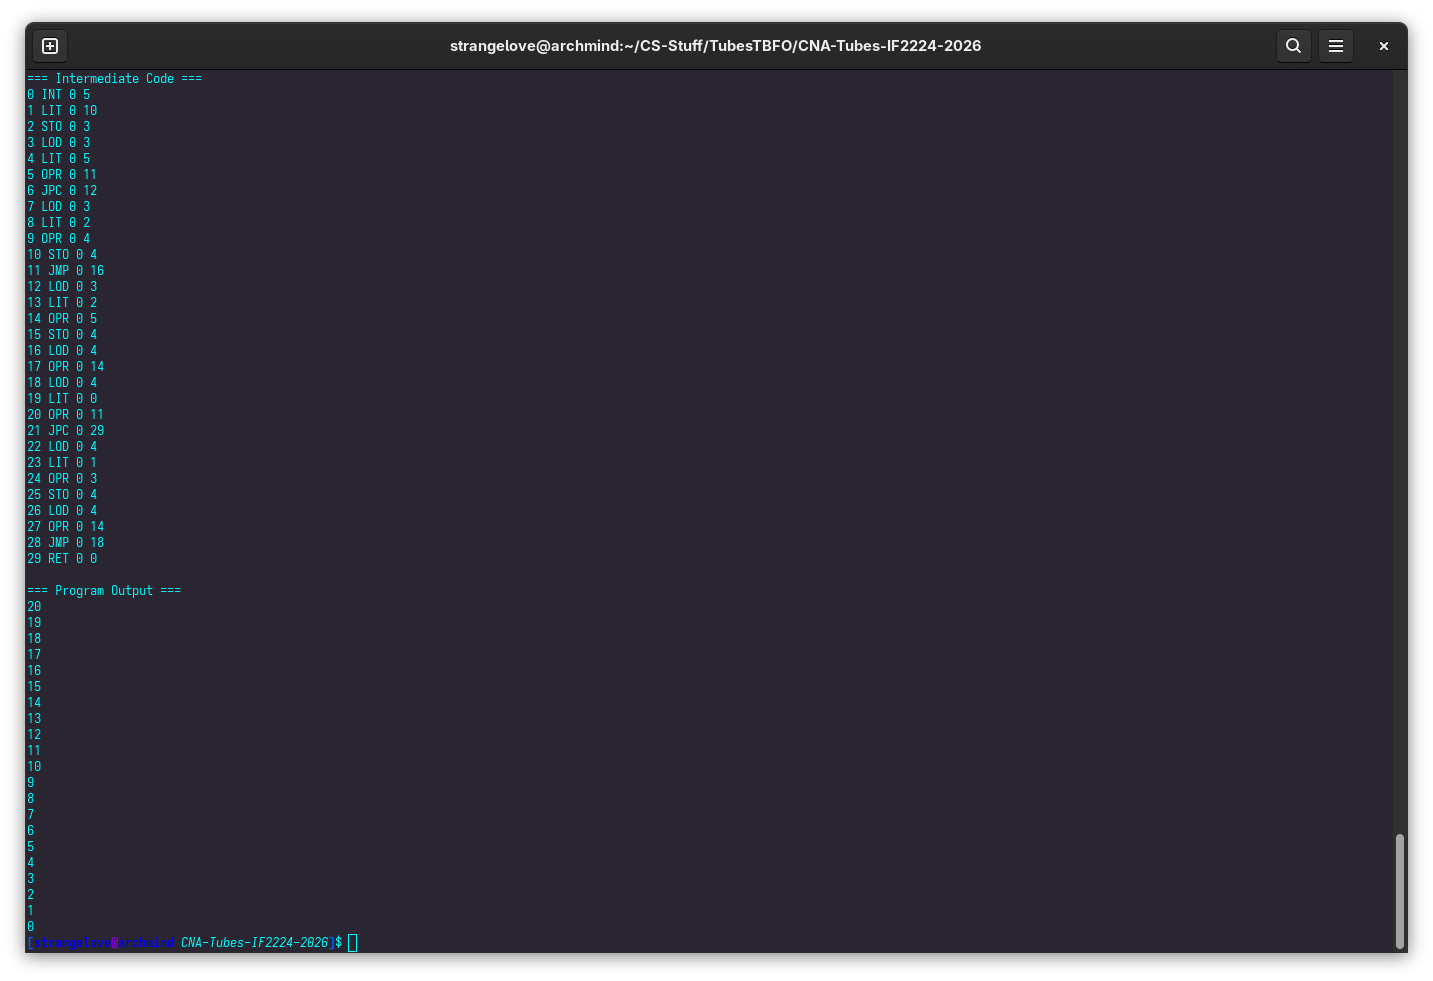
\includegraphics[width=15cm]{gambar/tc4_src_testkeywords.png}
\end{center}

\textbf{Analisis.} Intermediate Code yang dihasilkan identik dengan contoh pada
spesifikasi. \texttt{JPC 0 13} melompati blok \texttt{then} bila kondisi salah,
\texttt{JMP 0 17} melewati blok \texttt{else}, dan \texttt{JMP 0 19} pada
perulangan kembali ke evaluasi kondisi---membuktikan translasi control flow tepat.

%------------------------------------------------------------------------------
\subsection{Kasus 5 -- Penanganan Error: Pembagian dengan Nol}

\textbf{Tujuan.} Memverifikasi bahwa kesalahan runtime tidak membuat program
\emph{crash}, melainkan ditangkap dan dilaporkan secara \emph{graceful}.

\begin{minipage}[t]{0.48\textwidth}
\textbf{Masukan} (\texttt{src\_divzero.txt}):
\begin{lstlisting}[style=kodeArion, numbers=none]
program DivByZero;
var
  a, b: integer;
begin
  a := 10;
  b := 0;
  writeln(a div b);
end.
\end{lstlisting}
\end{minipage}\hfill
\begin{minipage}[t]{0.48\textwidth}
\textbf{Intermediate Code:}
\begin{lstlisting}[style=kodeTAC, numbers=none]
1 INT 0 5
2 LIT 0 10
3 STO 0 3
4 LIT 0 0
5 STO 0 4
6 LOD 0 3
7 LOD 0 4
8 OPR 0 5     ; a div b
9 OPR 0 14
10 RET 0 0
\end{lstlisting}
\end{minipage}

\textbf{Keluaran Program:}
\begin{lstlisting}[style=kodeTAC, numbers=none]
[ERROR] DivisionByZeroError: division by zero !
\end{lstlisting}

\begin{center}
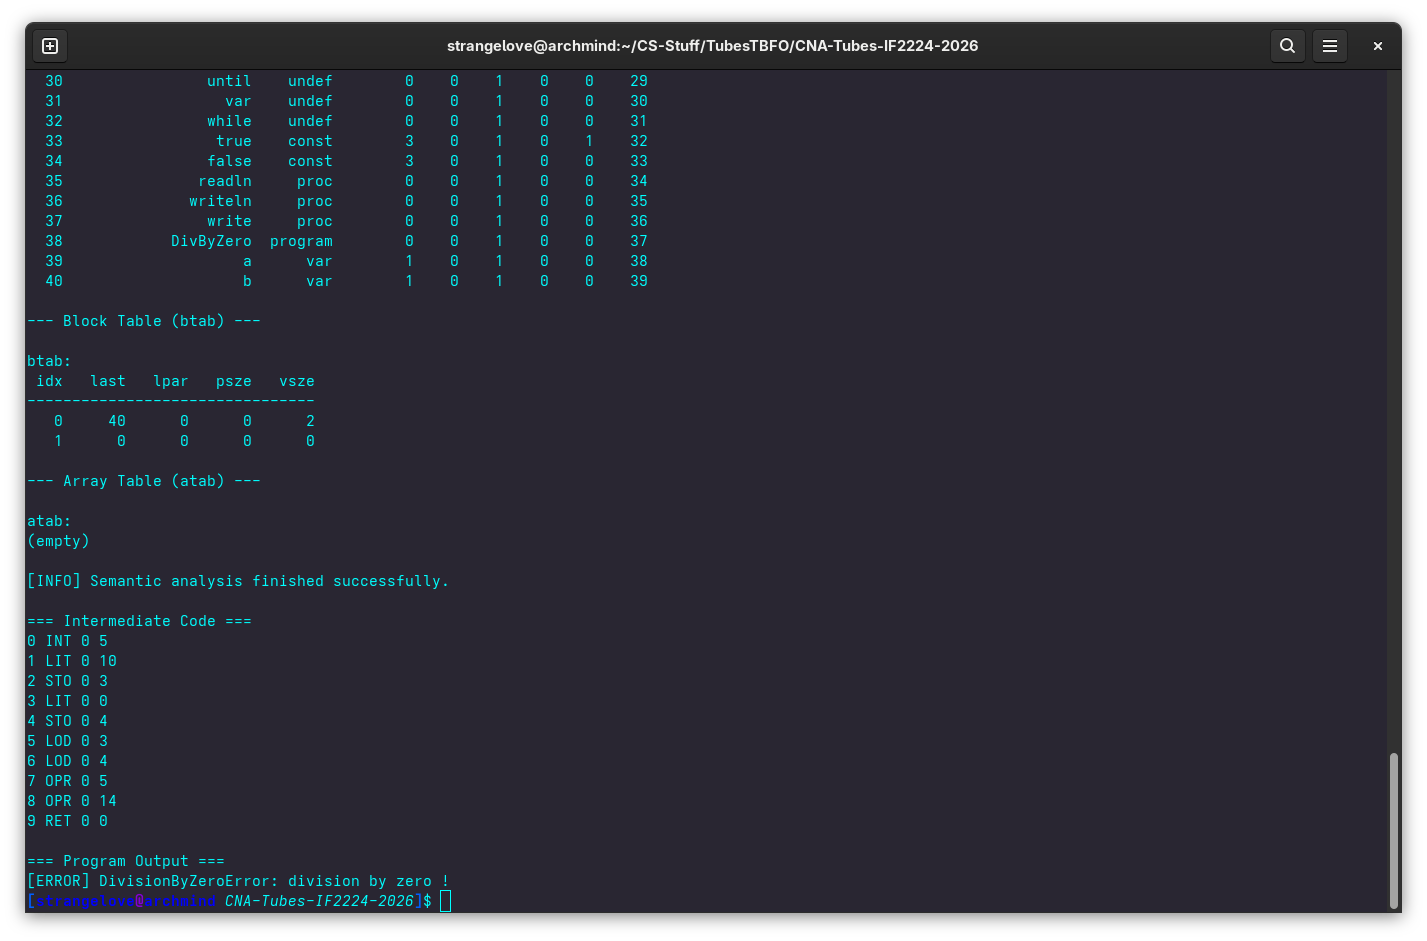
\includegraphics[width=15cm]{gambar/tc5_src_divzero.png}
\end{center}

\textbf{Analisis.} Saat \texttt{DIV} (OPR 5) mendeteksi pembagi bernilai nol,
\texttt{RuntimeErrorHook::divisionByZero()} melempar \texttt{RuntimeError} yang
ditangkap \texttt{Interpreter::run()}. Program berhenti dengan pesan jelas, bukan
\emph{segmentation fault}.

%------------------------------------------------------------------------------
\subsection{Kasus 6 -- Penanganan Error: Numerical Overflow}

\textbf{Tujuan.} Menguji deteksi \emph{integer overflow} pada operasi aritmatika
sebelum nilai sempat membungkus (\emph{wrap-around}).

\begin{minipage}[t]{0.48\textwidth}
\textbf{Masukan} (\texttt{src\_overflow.txt}):
\begin{lstlisting}[style=kodeArion, numbers=none]
program NumericOverflow;
var
  big, hasil: integer;
begin
  big := 4000000000;
  hasil := big * big;
  writeln(hasil);
end.
\end{lstlisting}
\end{minipage}\hfill
\begin{minipage}[t]{0.48\textwidth}
\textbf{Intermediate Code:}
\begin{lstlisting}[style=kodeTAC, numbers=none]
1 INT 0 5
2 LIT 0 4000000000
3 STO 0 3
4 LOD 0 3
5 LOD 0 3
6 OPR 0 4     ; big * big
7 STO 0 4
8 LOD 0 4
9 OPR 0 14
10 RET 0 0
\end{lstlisting}
\end{minipage}

\textbf{Keluaran Program:}
\begin{lstlisting}[style=kodeTAC, numbers=none]
[ERROR] OverflowError: 'MUL' result exceeds the maximum integer value !
\end{lstlisting}

\begin{center}
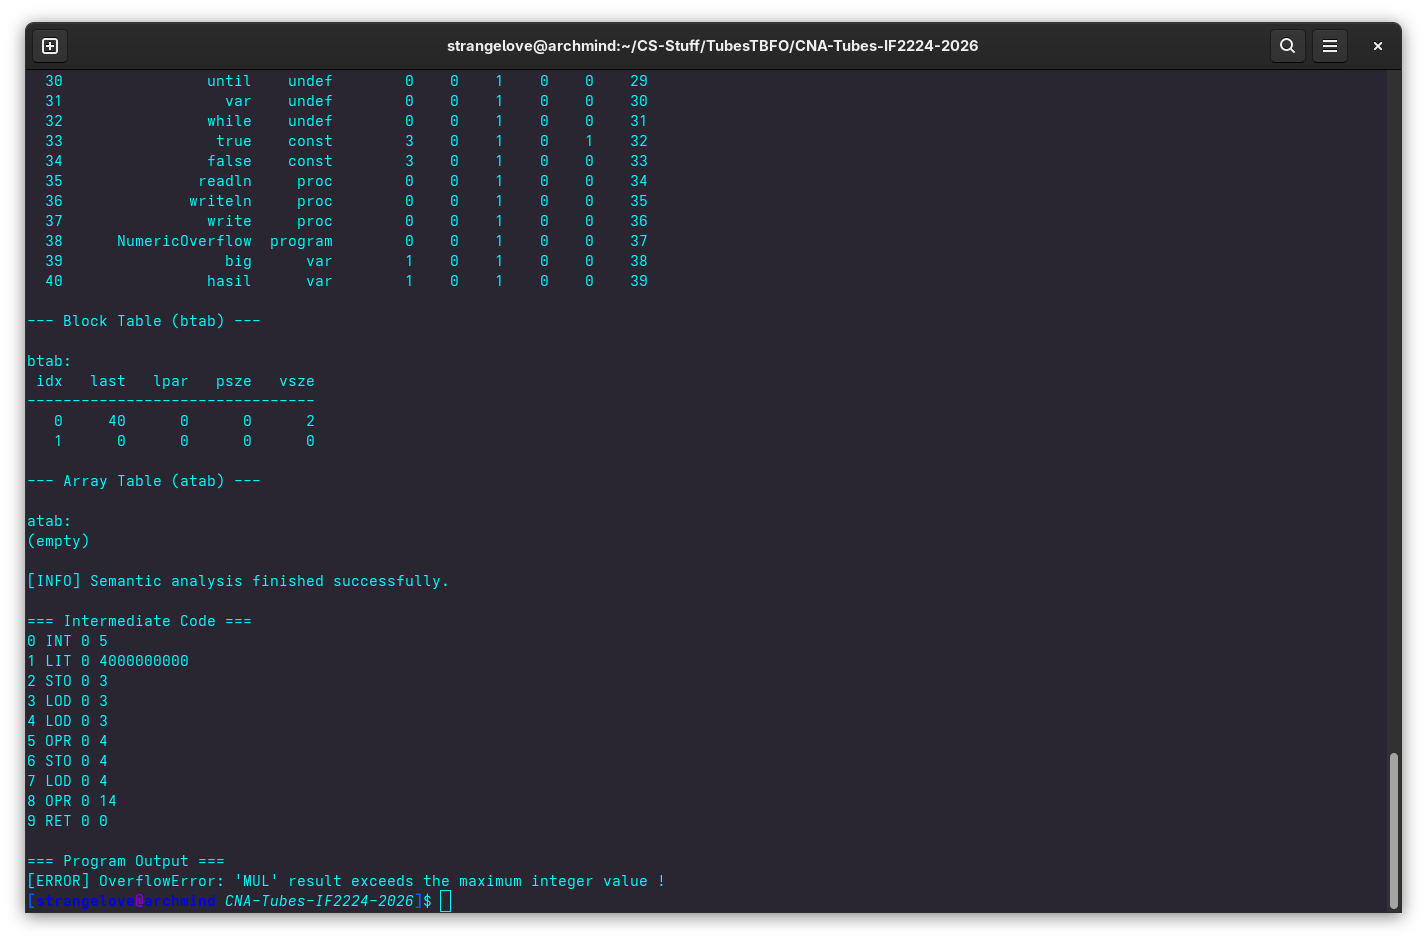
\includegraphics[width=15cm]{gambar/tc6_src_overflow.png}
\end{center}

\textbf{Analisis.} $4{,}000{,}000{,}000^2 = 1.6 \times 10^{19}$ melampaui batas
maksimum integer. \texttt{mulChecked} mendeteksinya melalui
\texttt{\_\_builtin\_mul\_overflow} dan melempar \texttt{OverflowError}, sehingga
hasil yang salah akibat \emph{wrap-around} tidak pernah dicetak.

%------------------------------------------------------------------------------
\subsection{Ringkasan Pengujian}

\begin{table}[H]
\centering
\caption{Ringkasan hasil pengujian Milestone 4.}
\renewcommand{\arraystretch}{1.2}
\begin{tabularx}{\textwidth}{@{}c X l c@{}}
\toprule
\textbf{No} & \textbf{Aspek yang Diuji} & \textbf{Keluaran} & \textbf{Status} \\
\midrule
1 & Penugasan \& cetak literal            & \texttt{10, 99}          & Sesuai \\
2 & Aritmatika \& relasional              & \texttt{10,24,4,TRUE,TRUE} & Sesuai \\
3 & Ekspresi bersarang \& modulus         & \texttt{56, 0}           & Sesuai \\
4 & Control flow IF-ELSE \& WHILE         & \texttt{20\dots0}        & Sesuai \\
5 & Error: pembagian dengan nol           & DivisionByZeroError      & Sesuai \\
6 & Error: numerical overflow             & OverflowError            & Sesuai \\
\bottomrule
\end{tabularx}
\end{table}

Keenam kasus uji memberikan hasil sesuai harapan. Generator menghasilkan
Intermediate Code yang valid (identik dengan contoh spesifikasi pada Kasus 4),
interpreter mengeksekusinya dengan benar, dan mekanisme keamanan runtime berhasil
menangkap kondisi error tanpa menyebabkan program \emph{crash}.

%==============================================================================
%  BAB IV - KESIMPULAN DAN SARAN
%==============================================================================
\section{Kesimpulan dan Saran}

\subsection{Kesimpulan}

Milestone 4 berhasil menyatukan seluruh komponen kompiler Arion yang dibangun pada
milestone sebelumnya menjadi sebuah kompiler yang utuh dan dapat dieksekusi. Dari
pengerjaan tahap ini dapat ditarik beberapa kesimpulan.

Pertama, \emph{Decorated AST} hasil analisis semantik berhasil diratakan menjadi
\emph{Three-Address Code} melalui penelusuran berbasis DFS. Ekspresi diterjemahkan
secara postorder sehingga operand selalu tersedia di stack sebelum operatornya
dijalankan, sementara struktur control flow \texttt{if-else} dan \texttt{while}
diratakan menggunakan kombinasi label dan instruksi lompat dengan konvensi
\emph{IF\_FALSE}. Intermediate Code yang dihasilkan terbukti identik dengan contoh
pada spesifikasi.

Kedua, interpreter berbasis \emph{stack machine} mampu mengeksekusi Intermediate
Code dengan benar melalui siklus \emph{fetch--decode--execute}, mengelola memori
dalam bentuk stack frame (static link, dynamic link, return address, dan variabel),
serta menghasilkan keluaran nyata program melalui operasi \texttt{WRT}/\texttt{WRTLN}.

Ketiga, aspek keamanan runtime---termasuk tantangan bonus---telah
diimplementasikan. Interpreter menangani pembagian dengan nol, overflow/underflow
aritmatika, stack overflow/underflow, stack corruption, stack smashing, akses
memori dan target lompat di luar batas, serta pemeriksaan tipe saat eksekusi.
Seluruh kondisi error dilaporkan secara \emph{graceful} dengan pesan informatif
tanpa membuat program \emph{crash}, sebagaimana ditunjukkan pada Kasus 5 dan 6.

Keempat, kode disusun secara modular dengan pemisahan tanggung jawab yang jelas
antara pembentukan kode (\texttt{intermediate/}) dan eksekusi
(\texttt{interpreter/}), dijembatani oleh pola \emph{adapter} sehingga kedua sisi
tetap terpisah (\emph{loosely coupled}).

\subsection{Saran}

Beberapa hal dapat dikembangkan lebih lanjut. Implementasi pemanggilan
fungsi/prosedur (\texttt{CAL}/\texttt{RET} dengan \emph{nested scope} dan
\emph{passing} argumen penuh) masih bersifat dasar dan dapat dilengkapi agar
mendukung rekursi serta variabel lokal antar-frame secara menyeluruh. Selain itu,
pembentukan kode dapat diperluas untuk menangani tipe data terstruktur seperti
\emph{array} dan \emph{record} beserta validasi indeks \emph{out-of-bounds} saat
runtime. Dari sisi optimasi, \emph{constant folding} dan eliminasi instruksi
redundan dapat ditambahkan pada tahap pembentukan TAC untuk menghasilkan kode yang
lebih ringkas. Terakhir, cakupan pengujian otomatis dapat diperluas dengan kerangka
uji regresi agar setiap perubahan dapat diverifikasi dengan cepat.

%==============================================================================
%  LAMPIRAN
%==============================================================================
\section{Lampiran}

\subsection{Tautan Release Repository GitHub}

Kode sumber lengkap kompiler Arion beserta release Milestone 4 tersedia pada
repositori GitHub berikut.

\begin{itemize}
  \item \textbf{Repositori:} \url{https://github.com/Nusss0/CNA-Tubes-IF2224-2026}
  \item \textbf{Release Milestone 4 (tag \texttt{v0.4.1}):}\\
        \url{https://github.com/Nusss0/CNA-Tubes-IF2224-2026/releases/tag/v0.4.1}
\end{itemize}

\subsection{Pembagian Tugas}

Pembagian tugas dan persentase kontribusi setiap anggota kelompok pada Milestone 4
dirangkum pada Tabel~\ref{tab:tugas}.

\begin{table}[H]
\centering
\caption{Pembagian tugas dan persentase kontribusi Milestone 4.}
\label{tab:tugas}
\renewcommand{\arraystretch}{1.3}
\begin{tabularx}{\textwidth}{@{}l c X c@{}}
\toprule
\textbf{Nama} & \textbf{NIM} & \textbf{Tugas Milestone 4} & \textbf{Kontribusi} \\
\midrule
Stevanus Agustaf Wongso & 13524020 &
Validasi runtime pada stack machine, modul \texttt{RuntimeErrorHook}, deteksi
overflow/underflow, stack corruption \& smashing, runtime type checking
(tantangan bonus). & 25\% \\
\addlinespace
Renuno Yuqa Frinardi & 13524080 &
Inti interpreter / stack machine (\texttt{StackMachine}, \texttt{RuntimeValue},
\texttt{RuntimeContext}), \texttt{TacAdapter}, dan penyusunan kasus uji
Milestone 4. & 25\% \\
\addlinespace
Valentino Daniel Kusumo & 13524104 &
Pembentukan control flow pada generator (\texttt{genIf}, \texttt{genWhile}) 
\& compound block, integrasi pipeline pada \texttt{main}, serta penulisan laporan. & 25\% \\
\addlinespace
Michael James Liman & 13524106 &
Inti \texttt{TacGenerator} (pemetaan alamat, pembentukan ekspresi \& penugasan,
resolusi label, pencetakan), kasus uji ekspresi/control flow, dan penulisan
laporan. & 25\% \\
\midrule
\multicolumn{3}{r}{\textbf{Total}} & \textbf{100\%} \\
\bottomrule
\end{tabularx}
\end{table}

%==============================================================================
%  REFERENSI
%==============================================================================
\section{Referensi}

\begin{enumerate}[label={[\arabic*]}]
  \item A. V. Aho, M. S. Lam, R. Sethi, dan J. D. Ullman, \textit{Compilers:
        Principles, Techniques, and Tools}, edisi ke-2. Boston: Addison-Wesley,
        2006.
  \item Tim Asisten IF2224, \textit{Spesifikasi Milestone 4 -- Tubes IF2224 TBFO:
        Intermediate Code and Interpreter}, Institut Teknologi Bandung, 2026.
  \item Tim Asisten IF2224, \textit{Lampiran Spesifikasi Milestone 4 -- Guidebook
        Konvensi Intermediate Code}, Institut Teknologi Bandung, 2026.
  \item P. Koopman, \textit{Stack Computers: The New Wave}. [Daring]. Tersedia:
        \url{https://users.ece.cmu.edu/~koopman/stack_computers/sec3_2.html}
  \item E. Bendersky, ``Stack frame layout on x86-64,'' 2011. [Daring]. Tersedia:
        \url{https://eli.thegreenplace.net/2011/09/06/stack-frame-layout-on-x86-64}
  \item GEPL, ``Decorated Abstract Syntax Tree,'' University of Minho. [Daring].
        Tersedia: \url{https://epl.di.uminho.pt/~gepl/GEPL_DS/Alma2/dapast.php}
\end{enumerate}


\end{document}
